\documentclass{article}
\usepackage{geometry}
\usepackage{graphicx}
\geometry{margin=1in}
\usepackage{amsmath}
\usepackage[english]{babel}
\usepackage[ruled,linesnumbered]{algorithm2e}
\usepackage{caption}
\usepackage{subcaption}

\title{}
\author{}

\begin{document}

\section{Q-Learning Agent}
\subsection{Softmax with temperature control}
\begin{figure}[h]
	\begin{subfigure}{0.5\textwidth}
		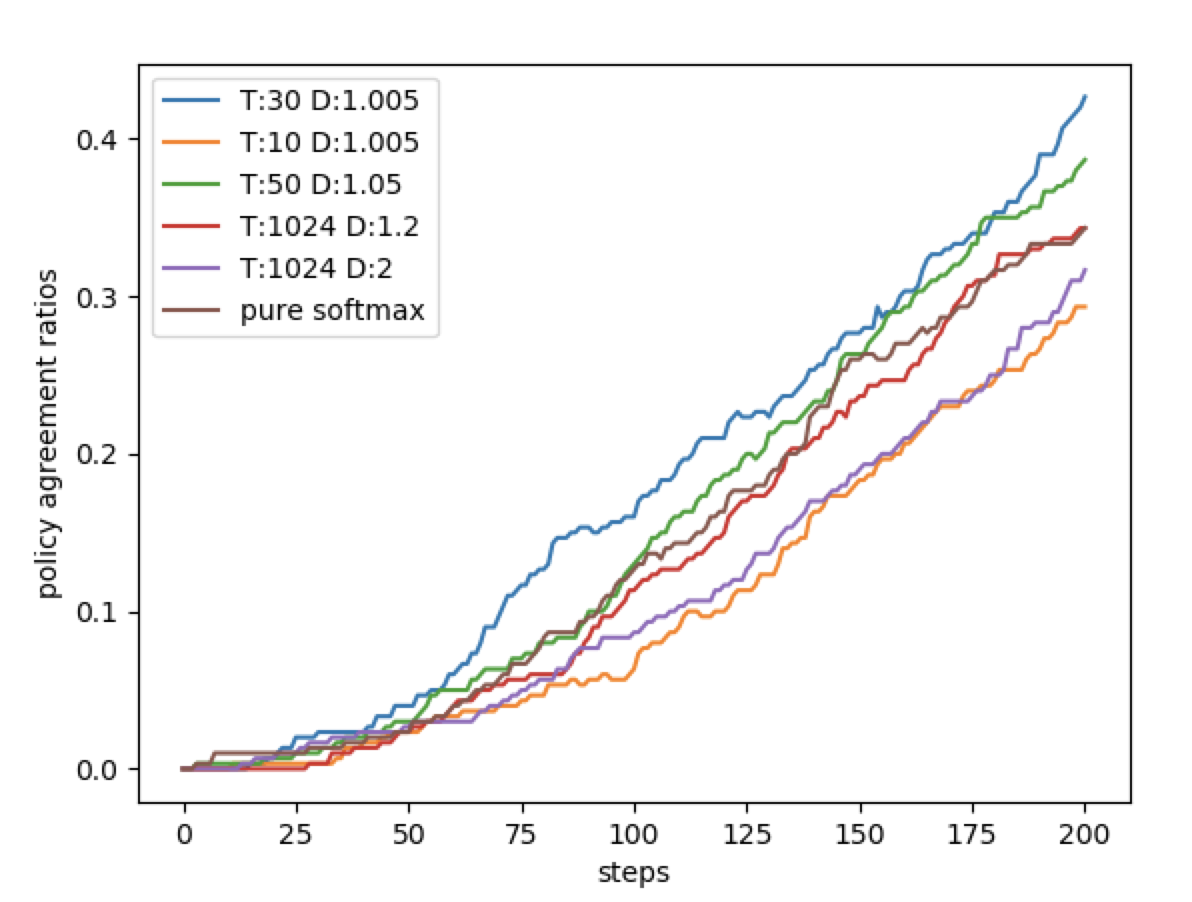
\includegraphics[width=0.9\linewidth, height=5cm]{images/temp_0_200.png} 
		\caption{}
	\end{subfigure}
	\begin{subfigure}{0.5\textwidth}
		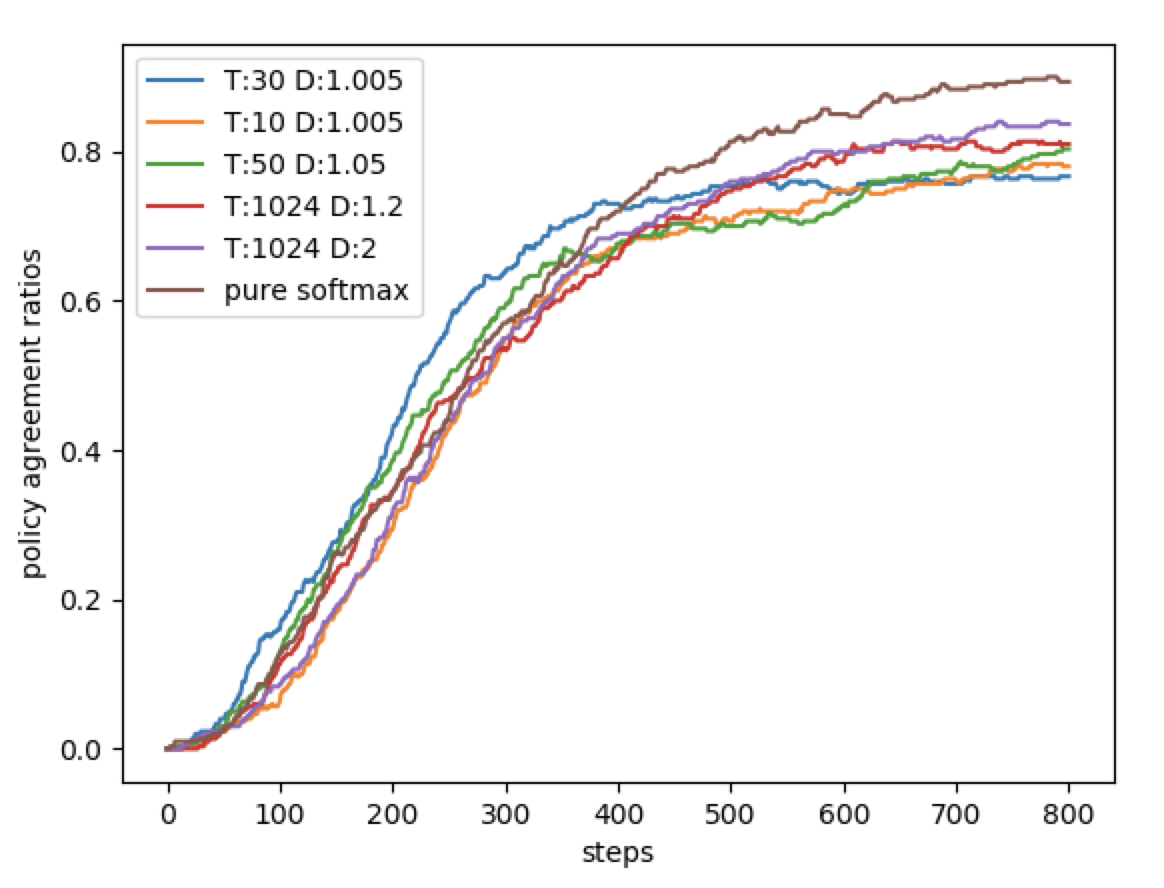
\includegraphics[width=0.9\linewidth, height=5cm]{images/temp_0_800.png}
		\caption{}
	\end{subfigure}
	\begin{subfigure}{0.5\textwidth}
		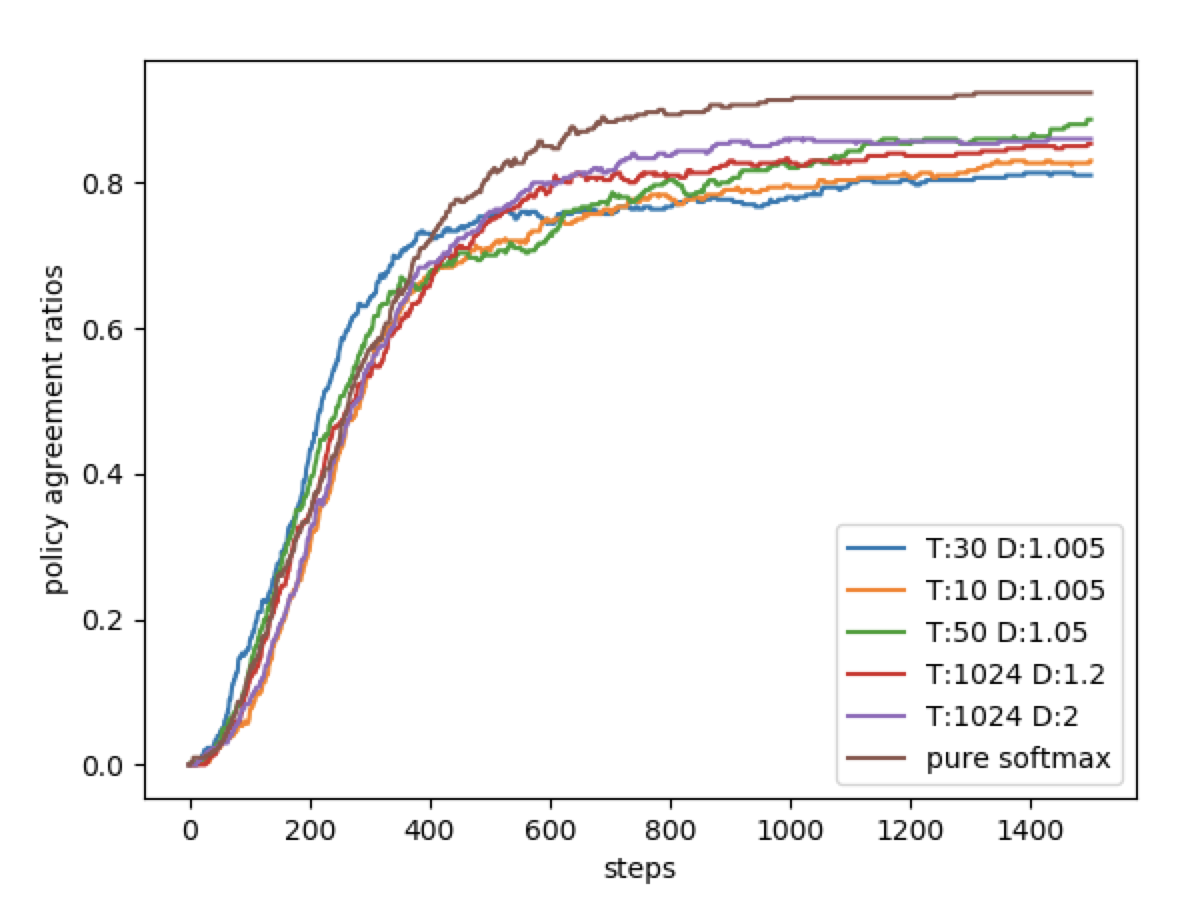
\includegraphics[width=0.9\linewidth, height=5cm]{images/temp_0_1500.png}
		\caption{}
	\end{subfigure}
	\begin{subfigure}{0.5\textwidth}
		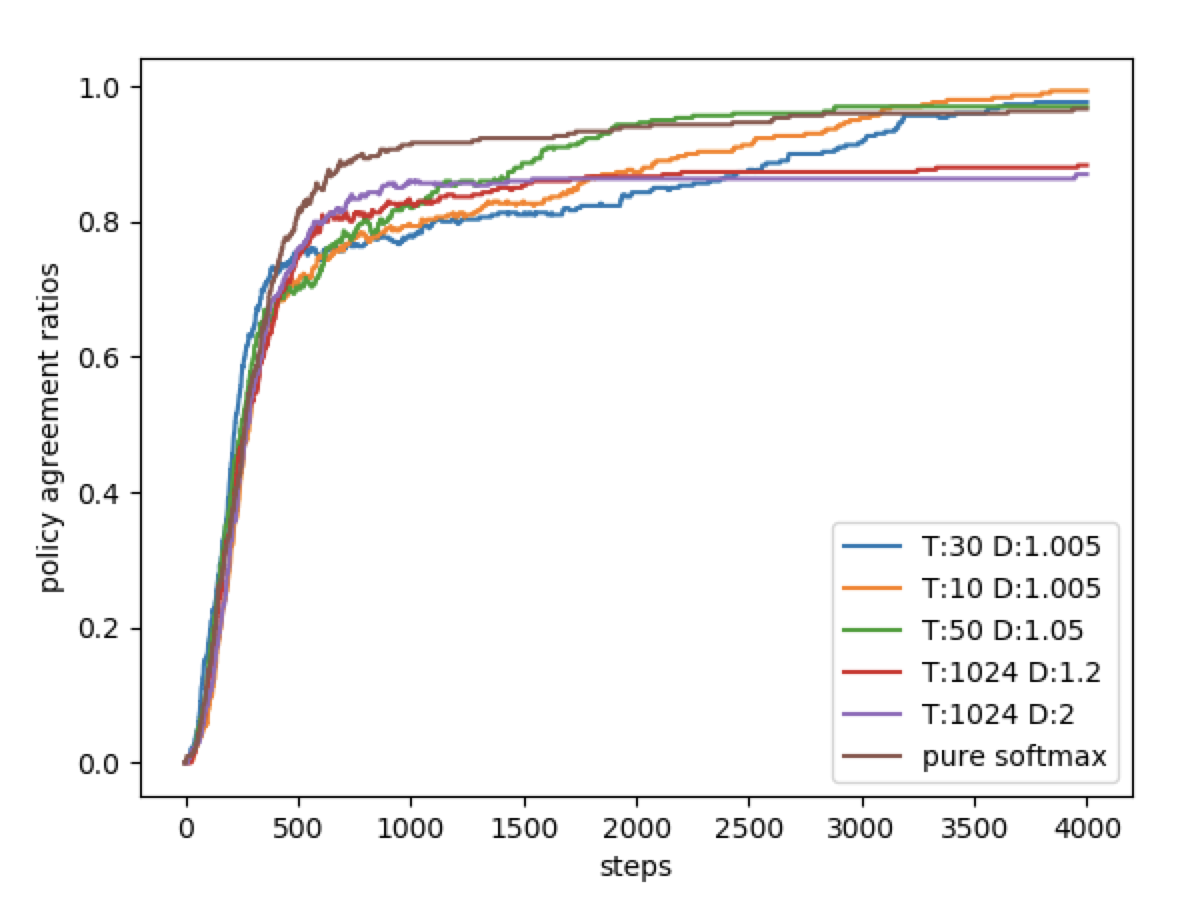
\includegraphics[width=0.9\linewidth, height=5cm]{images/temp_0_4000.png}
		\caption{}
	\end{subfigure}
	\caption{Average policy agreement ratios at each time step of experiments with different temperature control strategy. T is the initial temperature and D is the temperature decreasing rate}
\end{figure}

In our experiments, we tested the q-learning agents using softmax with different temperature control in the gridworld. Each agent was tested for 20 times in the same environment and the average policy agreement ratio at each time step was recorded. The result shown in Figure 1 illustrates that no method is significantly outperform the others. All of them took a long time to improve their policy after reaching 90 percent accuracy; some of them like agents with large decreasing rate (D=1.2 and D=2) even failed to reach policy agreement. The reason is that after running for a long time (over 1000 steps), the temperature has decreased to a sufficiently low value, which causes the agent to keep taking its suboptimal actions greedily without exploring other options.


\subsection{Epsilon-Greedy}
\begin{figure}[h]
	\begin{subfigure}{0.5\textwidth}
		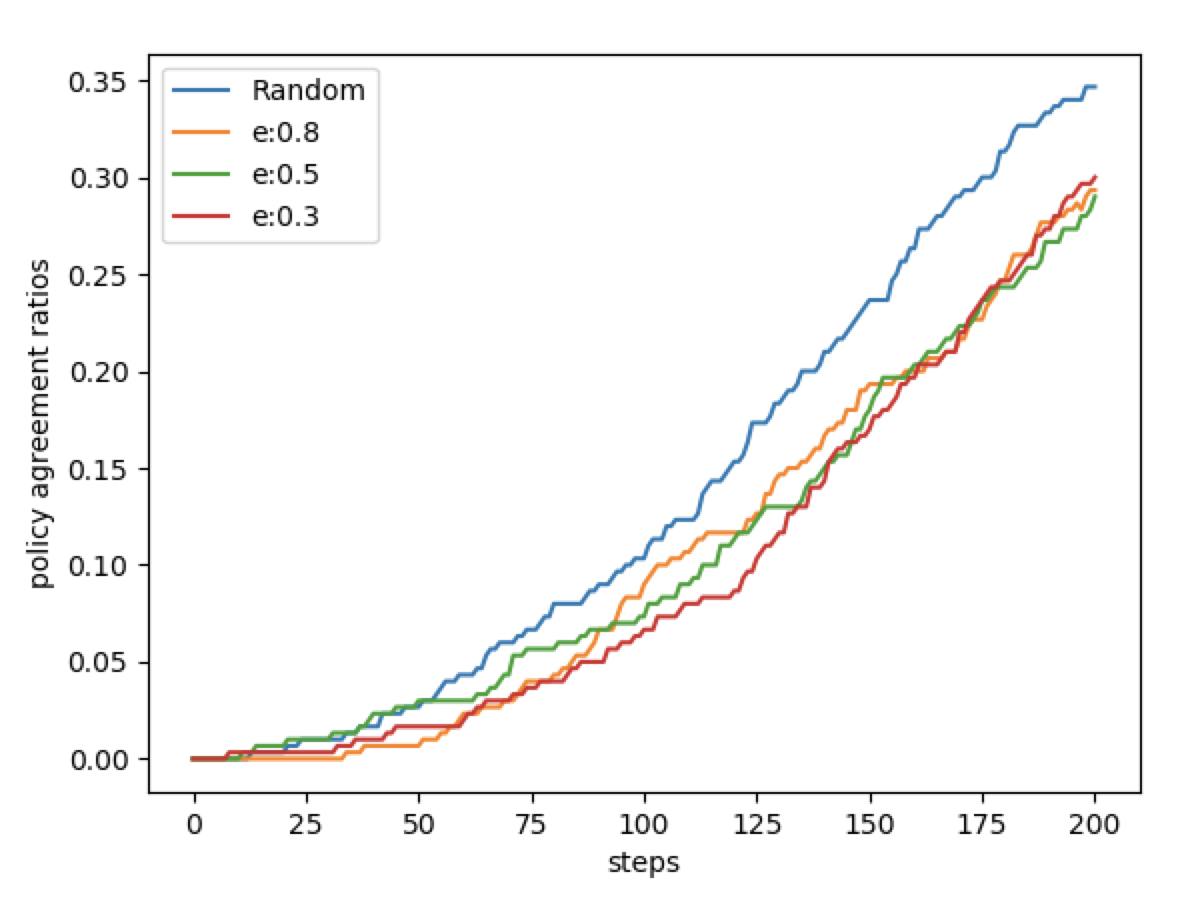
\includegraphics[width=0.9\linewidth, height=5cm]{images/epsilon_0_200.png} 
		\caption{}
	\end{subfigure}
	\begin{subfigure}{0.5\textwidth}
		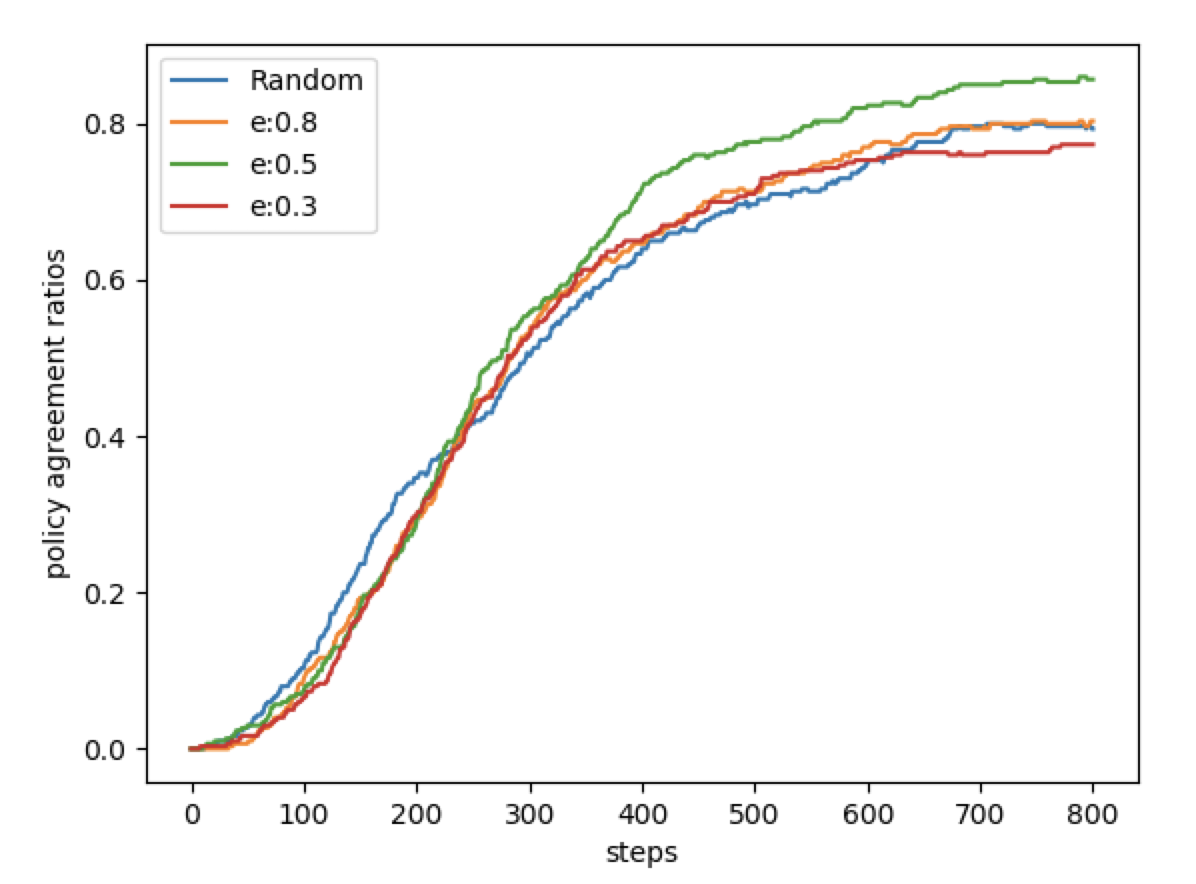
\includegraphics[width=0.9\linewidth, height=5cm]{images/epsilon_0_800.png}
		\caption{}
	\end{subfigure}
	\begin{subfigure}{0.5\textwidth}
		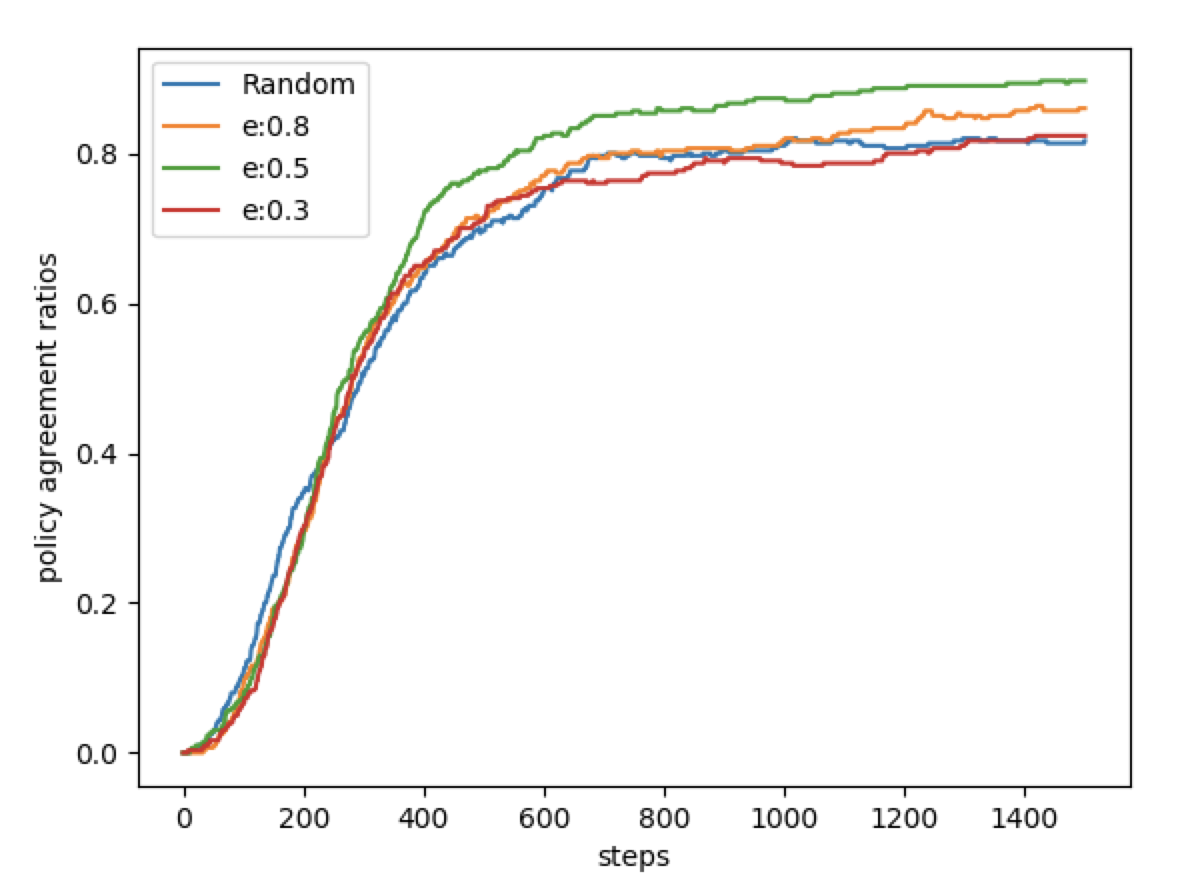
\includegraphics[width=0.9\linewidth, height=5cm]{images/epsilon_0_1500.png}
		\caption{}
	\end{subfigure}
	\begin{subfigure}{0.5\textwidth}
		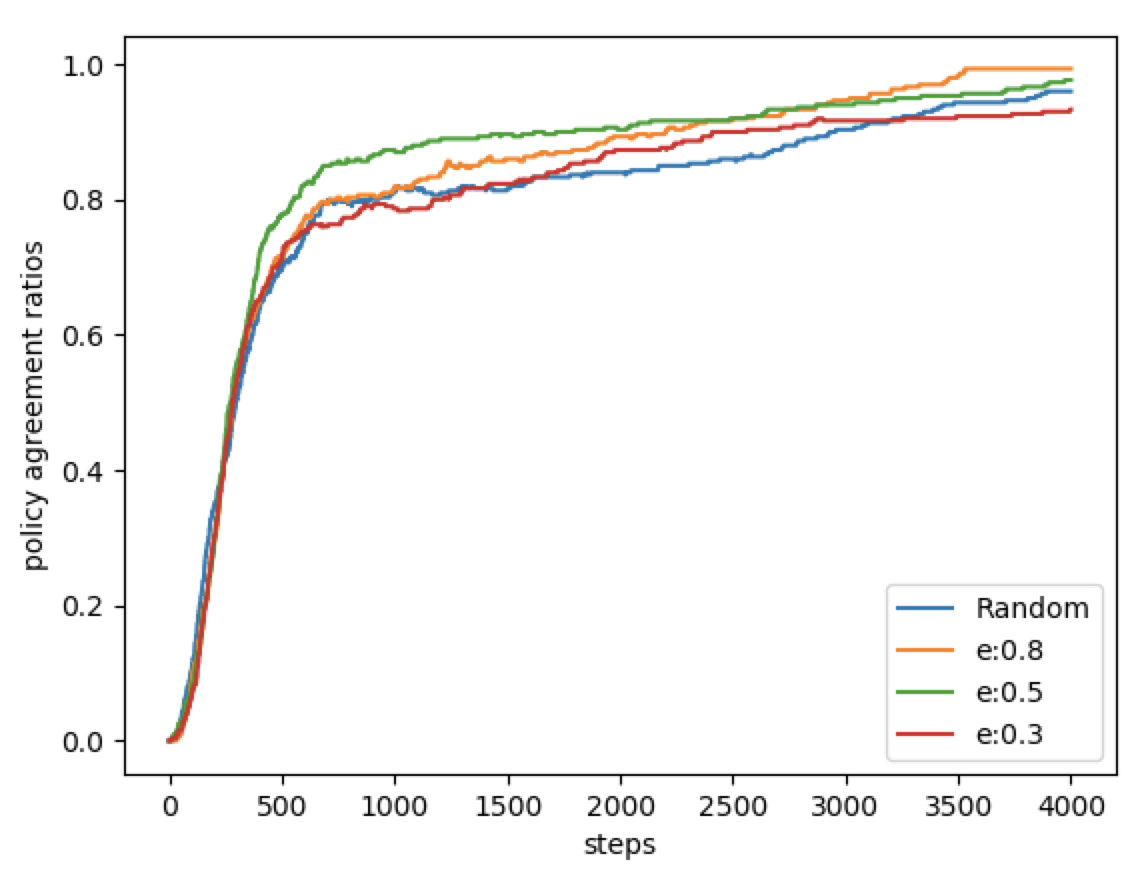
\includegraphics[width=0.9\linewidth, height=5cm]{images/epsilon_0_4000.png}
		\caption{}
	\end{subfigure}
	\caption{Average policy agreement ratios at each time step of experiments with different epsilon values.}
\end{figure}

Similar to the softmax-agent experiments, we tested each agent with different epsilon value in the same environment for 20 times and recorded the average policy agreement ratio at each time step. There is also no method significantly better than the others. The agent with e=0.5 might reach 80 percent agreement more quickly than others in the first 1000 steps, but the agents with higher degree of randomness might reach a similar or even better agreement ratio eventually.


\subsection{Comparison}
\begin{figure}[h]
	\begin{subfigure}{0.5\textwidth}
		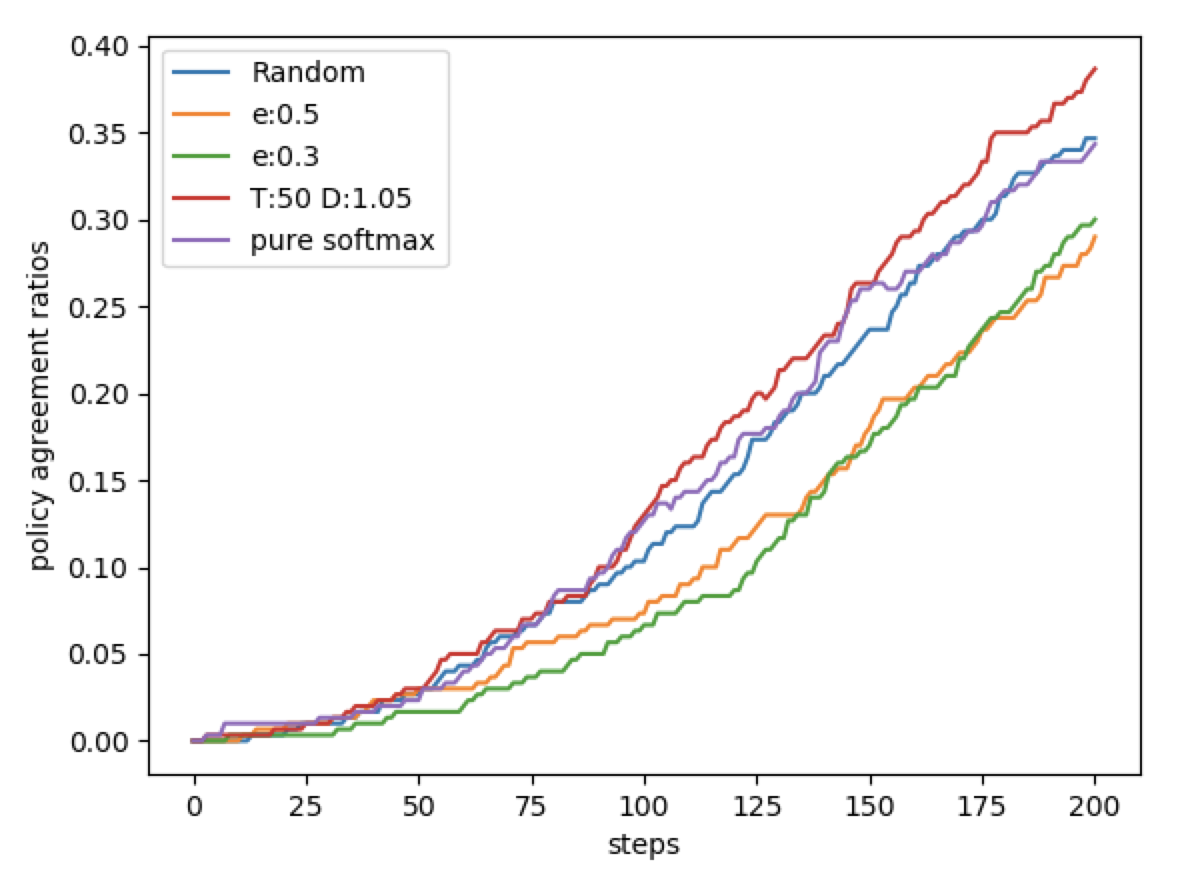
\includegraphics[width=0.9\linewidth, height=5cm]{images/both_0_200.png} 
		\caption{}
	\end{subfigure}
	\begin{subfigure}{0.5\textwidth}
		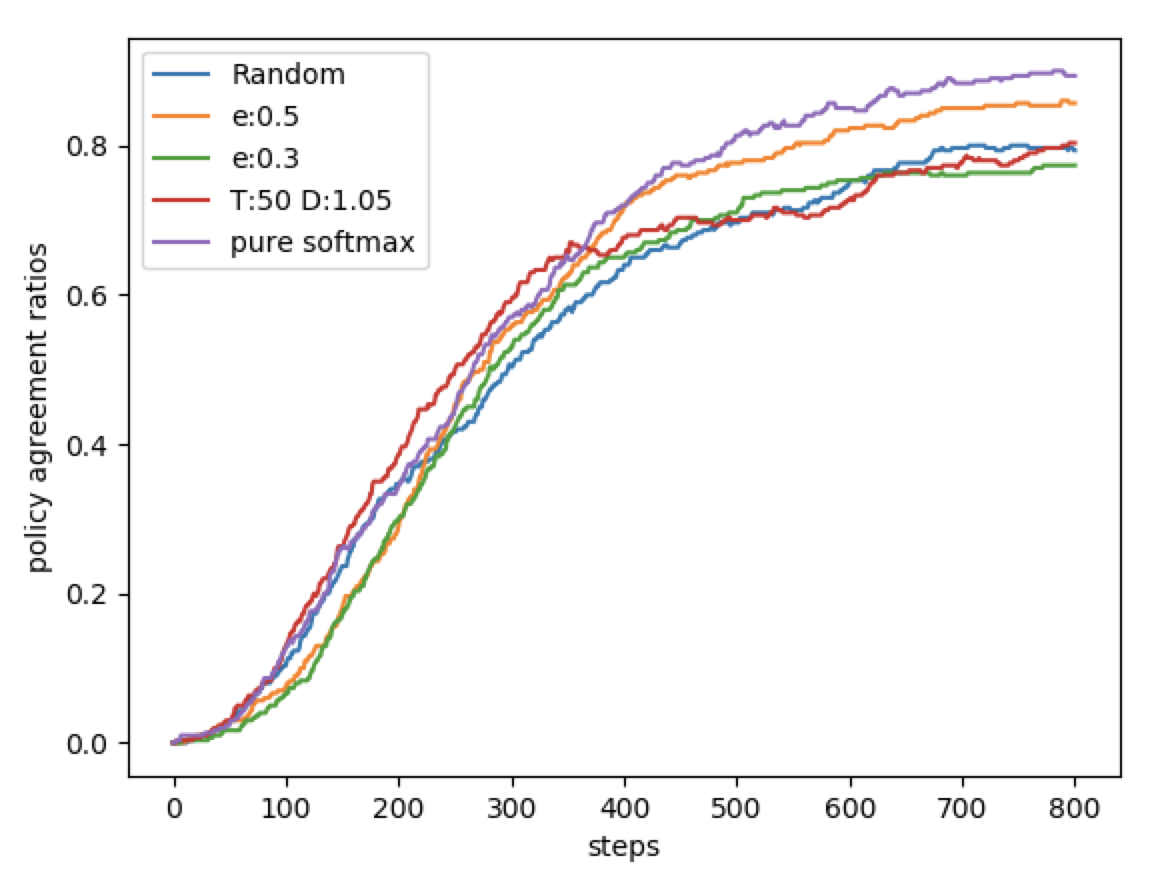
\includegraphics[width=0.9\linewidth, height=5cm]{images/both_0_800.png}
		\caption{}
	\end{subfigure}
	\begin{subfigure}{0.5\textwidth}
		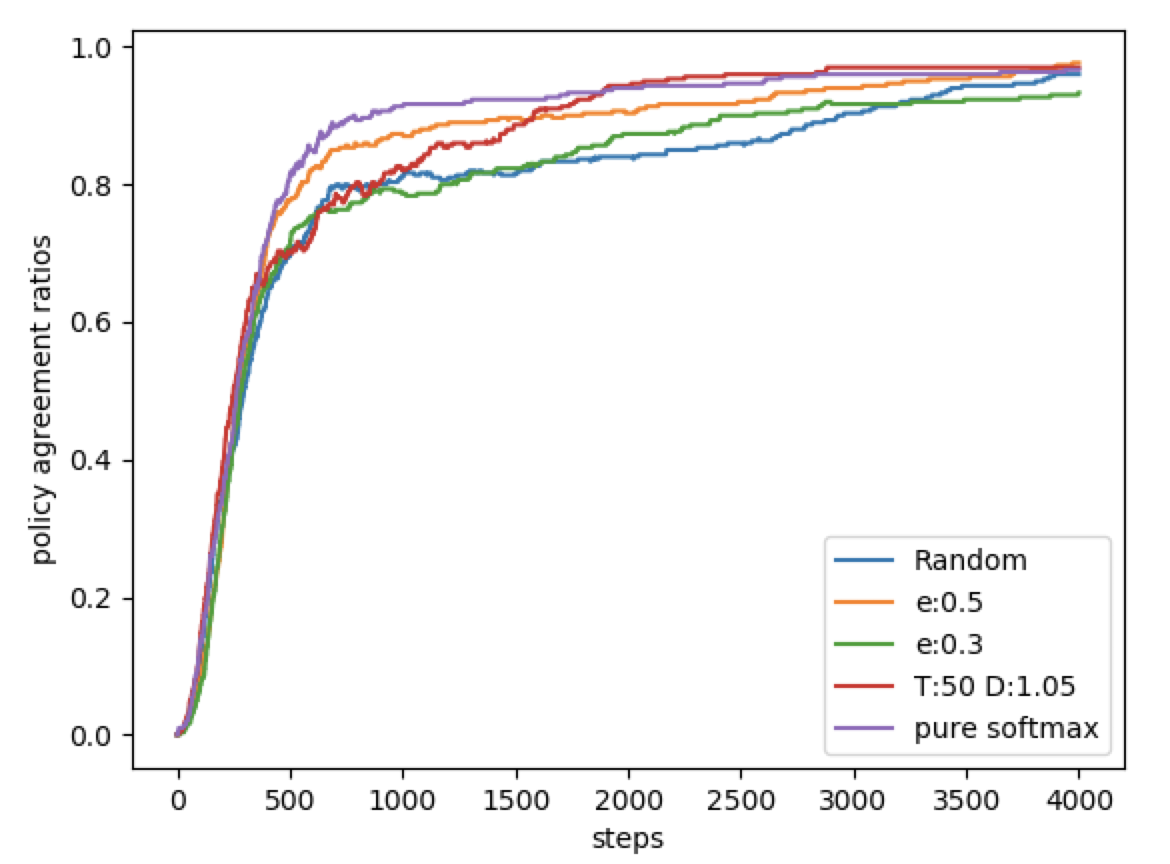
\includegraphics[width=0.9\linewidth, height=5cm]{images/both_0_4000.png}
		\caption{}
	\end{subfigure}
	\caption{Comparisons among q-learning agents with different settings.}
\end{figure}

Both of softmax and e-greedy agents suffer from slow improvement after reaching approximately 80 percent agreement. In addition, they both have the issue of slow start. The increasing slope of the graph at the beginning stages shows that the goal is reached slowly at the beginning. These two issues are the two main factors that prevent the agent from learning the optimal policy efficiently in the gridworld. In the following TAMER experiment, we choose to use pure softmax as the exploration strategy, since it has relatively better performance in the early stages (before 1500 steps).


\section{Tamer Agent}
\begin{figure}[h]
	\begin{subfigure}{0.5\textwidth}
		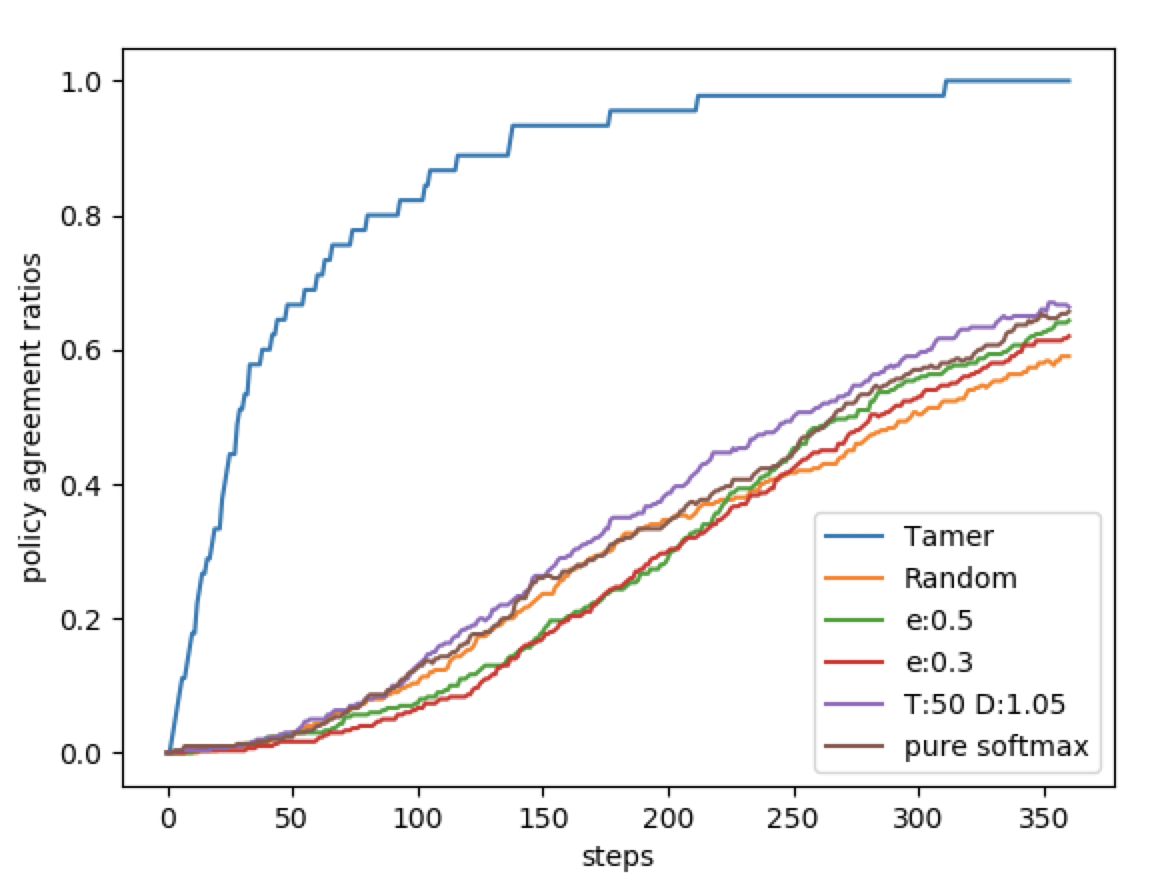
\includegraphics[width=0.9\linewidth, height=5cm]{images/all_0_400.png} 
		\caption{}
	\end{subfigure}
	\begin{subfigure}{0.5\textwidth}
		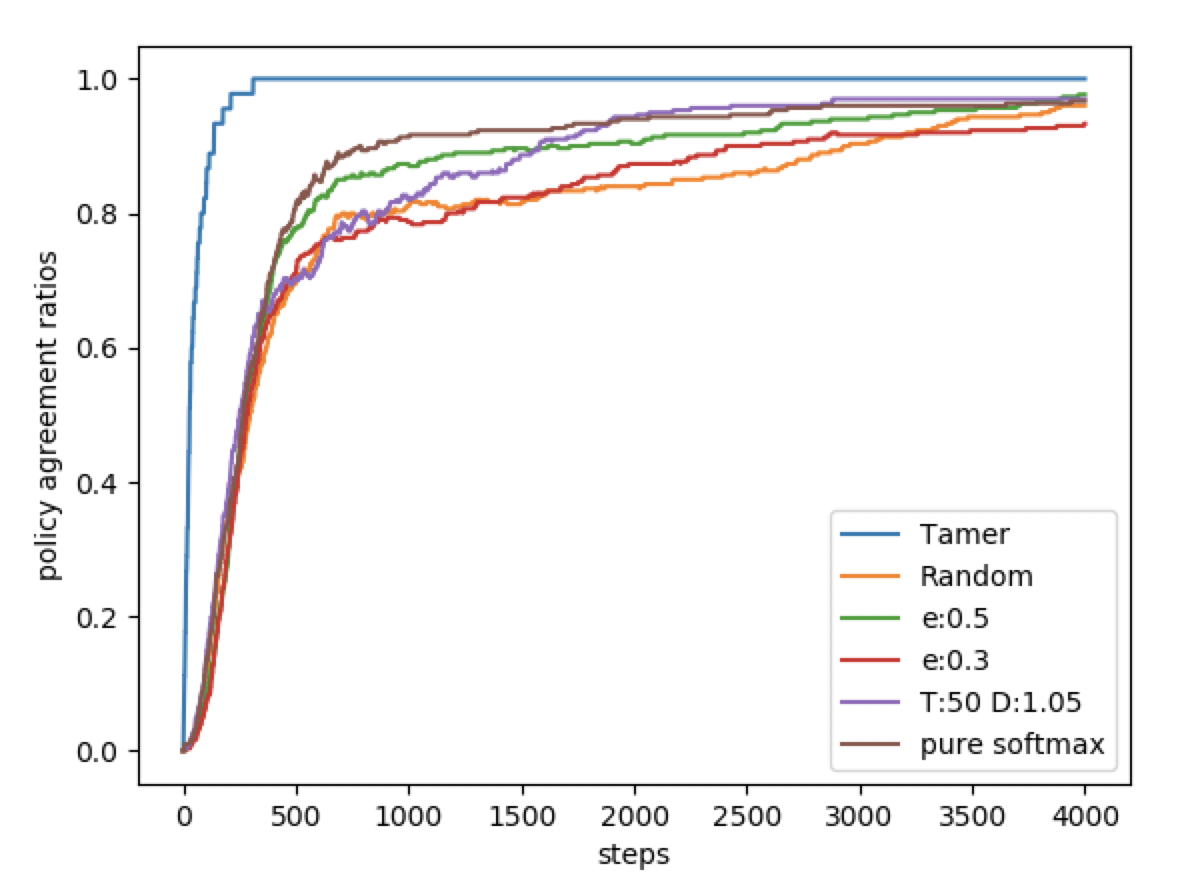
\includegraphics[width=0.9\linewidth, height=5cm]{images/all_0_4000.png}
		\caption{}
	\end{subfigure}
	\caption{Comparisons between Tamer agent and q-Learning agents.}
\end{figure}

TAMER outperforms all the other methods on the gridworld dramatically. From the graph, it can be noticed that the human knowledge greatly improves the learning efficiency at the early stages. By studying records, we can easily find that human signals help prevent the agent from searching for the goals blindly at the beginning. That is the reason why Tamer agent won't suffer from the slow start. However, due to the limitation of exploration strategy, the Tamer agent still has the issue of slow convergence after reaching 90 percent agreement.

\end{document}








